\documentclass{article}
\PassOptionsToPackage{table}{xcolor}
\PassOptionsToPackage{numbers}{natbib}
\usepackage{iclr2027_conference,times}
\input{math_commands.tex}
\usepackage{amsmath,amssymb}
\usepackage{booktabs}
\usepackage{graphicx}
\usepackage{xcolor}
\usepackage{array}
\usepackage{tabularx}
\usepackage{enumitem}
\usepackage{microtype}
\usepackage{hyperref}
\usepackage{url}
\setcitestyle{numbers,square,citesep={,}}
\raggedbottom

\definecolor{ink}{HTML}{25313B}
\definecolor{muted}{HTML}{5F6B75}
\definecolor{accent}{HTML}{EAF3F0}
\definecolor{accentblue}{HTML}{EEF4F8}
\definecolor{rulegray}{HTML}{D7DEE3}
\definecolor{proposed}{HTML}{EAF4F7}

\hypersetup{
  pdftitle={VoxReason: Listener-Independent Evaluation of Source-Grounded Speech Planning Before Synthesis},
  pdfauthor={Anonymous Authors},
  colorlinks=true,
  linkcolor=ink,
  citecolor=ink,
  urlcolor=ink
}

\setlist{nosep,leftmargin=*}
\renewcommand{\arraystretch}{1.12}
\newcolumntype{Y}{>{\raggedright\arraybackslash}X}
\newcommand{\repo}{the anonymous repository}
\newcommand{\metric}[1]{\textsc{#1}}

\title{VoxReason: Listener-Independent Evaluation of Source-Grounded Speech Planning Before Synthesis}
\author{Anonymous Authors\\
Anonymous Institution}
\date{}

\begin{document}
\maketitle
\lhead{VoxReason preprint}
\fancyfoot[C]{\small\thepage}
\thispagestyle{fancy}

\begin{abstract}
Speech systems increasingly infer how an utterance should be delivered from context, but a plausible plan can still be unsupported by the available evidence. VoxReason is a public benchmark and verifier package for testing this failure before waveform synthesis. Each case fixes the utterance, exposes a small set of derived source-label records, and changes one licensed cue at a time. A system must cite the record that supports its decision, fill a structured delivery plan, and change only the fields linked to the edited cue. The released source-label suite contains 100 cases split into 67 training, 17 development, and 16 test cases. We report deterministic, reproducible measurements, not a model leaderboard: a text-only control reaches 0.857 evidence F1, 0.185 plan-slot accuracy, and 0.427 citation-required grounded score, while a source-label oracle reaches 1.000 on each task by construction. Decisive-cue recall is 0.000 for the text-only control and 1.000 for the oracle reference; this contrast identifies the information exposed to a learned planner by the source-label task. Anti-shortcut checks show why source-emotion priors are insufficient: on a source-key-disjoint holdout, a prior-only predictor reaches 0.958 plan-slot accuracy but has zero counterfactual consistency. VoxReason therefore supplies a narrow, auditable measurement layer for source-grounded speech planning. It does not evaluate listener judgments, rendered speech quality, or broad waveform understanding.
\end{abstract}

\section{Introduction}

Speech generation systems are moving from fixed style controls toward context-aware decisions about delivery. A planner may need to infer whether a line should sound calm or urgent, how much pitch movement is appropriate, and which part of the context licenses that choice. Recent speech and audio language models connect language models to speech representations and generation tools \cite{speechgpt,audiogpt}, while newer work studies reasoning traces and context-aware text-to-speech \cite{thinksound,cottts}. These systems make the planning stage increasingly important: errors in the plan can be hidden by a fluent waveform, and a fluent waveform does not establish that the underlying decision was supported by the input.

The evaluation gap is specific. Existing audio benchmarks often ask for an answer about an audio clip or evaluate the quality of a generated waveform. Broad reasoning suites such as MMAR measure multi-step audio understanding across many domains \cite{mmar}. Codec and synthesis work likewise focuses on semantic preservation or output quality \cite{codec}. These settings are valuable, but they do not isolate whether a planner used the correct source evidence when the utterance is held constant and one contextual cue changes. Without that control, a system can exploit a stable text, speaker, or emotion prior and still appear context-aware.

VoxReason addresses this gap with a listener-independent measurement protocol. The benchmark is listener-independent because its primary score requires no human listening judgments: it measures source attribution and plan consistency before synthesis. This label does not claim that speech quality or listener preference is irrelevant; those questions remain outside the current score. Each case contains a fixed target utterance, contextual metadata, source-label cues, an expected plan, and a counterfactual edit. The verifier checks evidence identity, plan slots, citation coverage, and locality of the change. The repository is available at \repo\footnote{The repository contains derived labels, prompts, plans, and verification code. It does not redistribute the original RAVDESS audio files.}.

This paper makes three contributions. First, it defines a controlled task for source-grounded speech planning in which the utterance is fixed and the licensed cue is changed. Second, it releases a compact source-label suite and an executable verifier with auditable metrics. Third, it reports construct-validity and anti-shortcut analyses that separate an oracle reference from learned-system performance. The resulting package is intentionally narrow: it establishes a measurement layer for planning claims and leaves listener studies, waveform synthesis, and large-scale audio benchmarking to future work.

\section{Related Work}

\paragraph{Speech and audio language models.}
SpeechGPT demonstrated a language-model architecture with cross-modal speech interaction \cite{speechgpt}, and AudioGPT organized audio understanding and generation through foundation-model tools \cite{audiogpt}. These systems motivate evaluation of intermediate decisions as multimodal capabilities expand. VoxReason is complementary to them: it does not introduce a new audio language model, and its primary test does not require waveform input. Instead, it asks whether a planner can ground a delivery decision in a supplied source record and update the decision when the record changes.

\paragraph{Reasoning benchmarks and structured generation.}
MMAR evaluates deep reasoning over speech, audio, music, and mixed content with a broad set of questions and reasoning layers \cite{mmar}. ThinkSound uses structured reasoning to guide audio generation and editing \cite{thinksound}, and the ISCSLP 2026 CoT-TTS challenge explicitly separates context understanding, reasoning output, and speech generation \cite{cottts}. VoxReason focuses on a narrower failure mode that these settings do not by themselves identify: unsupported or uncited evidence in a structured speech plan. The benchmark is consequently easier to audit and less expressive than a full audio benchmark, but its intervention is more targeted.

\paragraph{Source data and acoustic representations.}
The case records are derived from the emotion and intensity labels of the Ryerson Audio-Visual Database of Emotional Speech and Song (RAVDESS) \cite{ravdess}. RAVDESS provides a controlled source for emotional speech, while VoxReason stores only derived labels, text prompts, source cues, and expected plans. This design makes the public package lightweight and keeps the acoustic preflight as a repository-level consistency check, not a perceptual result. Work on semantic audio codecs highlights the importance of preserving meaning through acoustic representations \cite{codec}; VoxReason tests a prior decision point, before a codec or synthesizer is involved.

\section{Task Formulation}

Let a case be
\begin{equation}
  x = (u, r, s, E, p^{\star}, \Delta),
\end{equation}
where $u$ is the target utterance, $r$ is a role profile, $s$ is a scene label, $E$ is a set of source-label evidence records, $p^{\star}$ is the expected delivery plan, and $\Delta$ is a one-cue counterfactual edit. A planner receives the case input and returns
\begin{equation}
  \hat{y} = (\hat{C}, \hat{p}, \hat{q}),
\end{equation}
where $\hat{C}$ is a set of cited evidence records, $\hat{p}$ is a structured plan, and $\hat{q}$ is an optional rationale. The rationale is not scored as free-form prose; the verifier scores the structured evidence and plan fields.

The plan contains seven scalar fields---emotion, intent, pitch, energy, rate, pause, and stance---plus a set-valued emphasis field. The counterfactual edit changes one source cue, such as an emotion-intensity label, while keeping the target text and the other case fields fixed. The expected plan delta specifies which plan fields are allowed to change. A grounded planner should satisfy three constraints:

\begin{enumerate}
  \item every cited record should be present in the case and match a gold evidence record;
  \item the plan should agree with the expected values across the eight scored slots; and
  \item after the edit, only the linked plan fields should change.
\end{enumerate}

This formulation distinguishes source grounding from surface plausibility. A system that emits the same plan for every cue may achieve high agreement on a biased split, but it fails the counterfactual locality test when the licensed cue changes.

\section{VoxReason Benchmark and Verifier}

\subsection{Released source-label suite}

The public suite contains 100 cases with 67 training cases, 17 development cases, and 16 test cases. It has two target utterances, one scene label, and two role labels. The source labels yield 15 unique emotion-intensity keys, and all 15 keys map deterministically to a single expected plan in the released construction. This determinism supports an auditable lookup oracle, but it also creates a meaningful shortcut risk, which we test explicitly. Table~\ref{tab:profile} summarizes the released scope.

\begin{table}[t]
\centering
\caption{Public source-label benchmark profile. Counts are taken from the released files and their deterministic construct-validity checks.}
\label{tab:profile}
\small
\begin{tabularx}{0.82\linewidth}{@{}Yr@{}}
\toprule
\textbf{Property} & \textbf{Value}\\
\midrule
Total cases & 100\\
Train / development / test & 67 / 17 / 16\\
Target utterances & 2\\
Scene labels & 1\\
Role labels & 2\\
Emotion-intensity keys & 15\\
Deterministic key mappings & 15 / 15\\
Valid gold plans under prompt taxonomy & 100 / 100\\
Public context-audio rows & 0\\
\bottomrule
\end{tabularx}
\end{table}

The suite is derived from RAVDESS source labels \cite{ravdess}. The public repository does not package raw licensed audio. Consequently, the main experiment is a source-label measurement and not an audio-input benchmark. The repository includes two separate consistency checks: an acoustic preflight over derived feature statistics and a source-label acoustic-anchor check over matched cases. These checks are useful for data auditing, but they do not support claims about listener perception or rendered speech quality.

\subsection{Verification path}

Figure~\ref{fig:overview} presents the full verification path. A case record supplies the utterance context and source-label cue. A typed planner selects delivery slots and cites the evidence it used. The verifier checks citation legality and slot agreement. A one-cue edit then changes a licensed cue while keeping other slots fixed. The final listener-independent checks report evidence coverage, citation-required grounding, and counterfactual locality. The waveform branch is outside the current claim scope.

\begin{figure}[t]
\centering
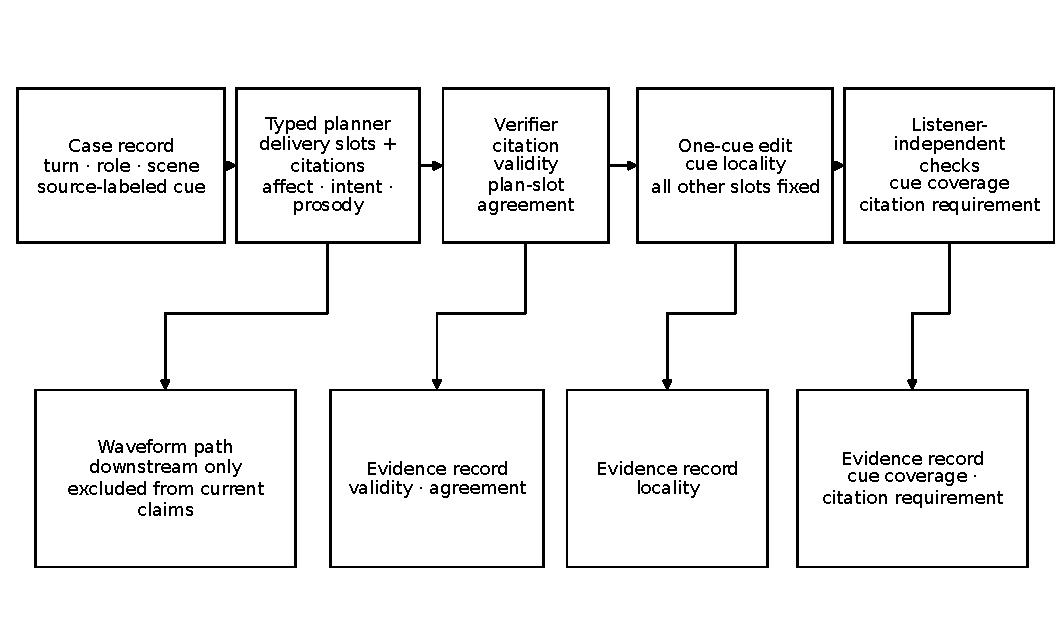
\includegraphics[width=\linewidth]{figures/revisions/pre_synthesis_schematic_v2/pre_synthesis_evidence_path.pdf}
\caption{VoxReason's pre-synthesis verification path. The benchmark evaluates a typed delivery plan and its cited source records. The lower ledger collects verifier evidence, while the dashed waveform branch is explicitly outside the current claims. The term ``listener-independent checks'' denotes pre-synthesis checks that do not require human listening judgments.}
\label{fig:overview}
\end{figure}

\subsection{Metrics}

For predicted evidence $\hat{C}$ and gold evidence $C^{\star}$, the verifier matches records by their stable cue identity and reports precision, recall, and F1. Let $m$ be the number of matched records. Then
\begin{equation}
 P = \frac{m}{|\hat{C}|}, \qquad R = \frac{m}{|C^{\star}|}, \qquad F_1 = \frac{2PR}{P+R}.
\end{equation}
The decisive-cue recall metric restricts the recall calculation to the cue changed by the counterfactual edit. Hallucinated evidence rate is $1-P$ when evidence is predicted, and uncited evidence rate is $1-R$ when gold evidence exists.

Plan-slot accuracy is the mean agreement over the seven scalar fields and the exact set match for emphasis:
\begin{equation}
 A_{\mathrm{plan}} = \frac{\sum_{j=1}^{7} \mathbf{1}[\hat{p}_j=p^{\star}_j] + \mathbf{1}[\hat{p}_{\mathrm{emph}}=p^{\star}_{\mathrm{emph}}]}{8}.
\end{equation}
The verifier's grounded score combines evidence F1, plan-slot accuracy, and the absence of hallucinated evidence:
\begin{equation}
 G = 0.45F_1 + 0.45A_{\mathrm{plan}} + 0.10(1-H),
\end{equation}
where $H$ is the hallucinated evidence rate. The citation-required grounded score applies the evidence recall gate:
\begin{equation}
 G_{\mathrm{cite}} = G R.
\end{equation}
This gate prevents a system from receiving a high grounded score when its plan is plausible but its supporting source records are missing.

For each counterfactual, the verifier compares the original and edited plans. A changed field is correct when it changes in the expected direction; an unrelated field is an unexpected change. Counterfactual consistency is the mean fraction of expected and forbidden changes handled correctly according to the repository implementation. We use the implementation as the normative definition and publish the code that computes it.

\section{Evaluation Protocol}

\subsection{Controlled information comparison}

The primary comparison uses the paired public source-label test cases. The text-only control receives the neutral textual context without the source-label evidence needed to identify the decisive cue. The source-label oracle receives the released gold evidence and gold plan; it is a deterministic reference point, not a learned model. Both systems are scored by the same verifier on the same 100 paired cases. The comparison therefore measures the information exposed by the source-label task and checks that the verifier responds to it as intended.

\subsection{Anti-shortcut checks}

The first check is leave-key-out construction validity. For each test key, the lookup is rebuilt after removing that key from the training cases. This removes the direct mapping that can make the released split easy. The second check uses a source-key-disjoint split with 60 training cases and 24 test cases. A prior-only predictor observes only the source emotion and never receives the full case record or a citation target. Its scores are calibration diagnostics, not benchmark performance. The purpose is to expose a failure mode in which a system predicts a stable emotion-conditioned plan while ignoring the intensity cue that should trigger the edit.

\subsection{Reproducibility and reporting}

All primary reported values in this paper are regenerated from the public repository with the following commands:

\begin{verbatim}
python3 scripts/check_benchmark_files.py
python3 scripts/reproduce_results.py
python3 -m pytest -q
\end{verbatim}

The first command checks the released checksums and case files. The second writes the compact result summaries, including the source-label construct-validity and source-key holdout reports. The test suite checks the benchmark files, scorer behavior, and summary invariants. When a result is reported, we name the split and the evidence condition. The learned-run files bundled with the repository are not used as a final model ranking because they contain incomplete prediction coverage; they are reported only as scorer-consistency diagnostics in Appendix~\ref{app:learned}.

\section{Results}

\subsection{The verifier exposes the source-grounding gap}

Table~\ref{tab:main-results} reports the paired source-label comparison. The text-only control obtains evidence F1 of 0.857, but its decisive-cue recall is 0.000. It achieves only 0.185 plan-slot accuracy and 0.427 citation-required grounded score. The source-label oracle reaches 1.000 on every positive metric and zero on hallucinated and uncited evidence by construction. The gap is the intended result: once the licensed source record is available, the verifier can detect the exact cue and its plan consequences. These values do not establish that a trained model can reach the oracle reference.

\begin{table}[t]
\centering
\caption{Paired public source-label measurement over 100 cases. The oracle line uses released gold evidence and gold plans, so it is a verifier reference and not learned-system performance. Higher is better for arrows up; lower is better for arrows down.}
\label{tab:main-results}
\small
\begin{tabularx}{\linewidth}{@{}Yrrrrrr@{}}
\toprule
\textbf{System} & \textbf{Ev. F1 $\uparrow$} & \textbf{Decisive $\uparrow$} & \textbf{Plan $\uparrow$} & \textbf{$G_{\mathrm{cite}}\uparrow$} & \textbf{Halluc. $\downarrow$} & \textbf{Uncited $\downarrow$}\\
\midrule
Text-only control & 0.857 & 0.000 & 0.185 & 0.427 & 0.000 & 0.250\\
\rowcolor{accent}
Source-label oracle & 1.000 & 1.000 & 1.000 & 1.000 & 0.000 & 0.000\\
\bottomrule
\end{tabularx}
\end{table}

The text-only control's zero hallucinated-evidence rate should be read together with its 0.250 uncited-evidence rate. It predicts only evidence that is legal when it predicts evidence, but it fails to cite one quarter of the gold evidence on average. The citation-required score captures that distinction by multiplying grounded quality by evidence recall. This is why $G_{\mathrm{cite}}$ is the primary aggregate for source-grounded claims.

\subsection{Evidence sensitivity under a source-key holdout}

The broader controlled matrix is reported in Table~\ref{tab:evidence-sensitivity}. It evaluates six conditions on 24 source-key-disjoint pairs for each of three deterministic seeds, for 432 valid records in total. The source-label oracle passes every verifier component, while the text evidence + declared delta control passes the locality checks only because the declared delta is supplied directly. This is a scorer sensitivity check, not evidence that a learned planner can infer the delta.

The text evidence-only and citation-echo controls retain perfect preservation of unrelated slots but have zero decisive-cue recall and zero required-change accuracy. The prior-only control reaches 0.958 original plan-slot accuracy, yet counterfactual consistency and required-change accuracy remain zero; its preservation rate is 0.667 and unexpected-change rate is 0.333. The result supplies a fail-closed claim gate: plan-slot agreement without decisive-cue recall and counterfactual locality cannot be called source-grounded planning. The shuffled-delta row is retained as a diagnostic, but its fixture has identical deltas and therefore does not provide an independent comparison.

\begin{table}[t]
\centering
\caption{Evidence-sensitivity matrix on the source-key-disjoint holdout. Each row contains 24 held-out pairs for each of three deterministic seeds (72 records total). The table reports the core claim-gate metrics; the complete locality summary, including preservation and unexpected-change rates, is in the released JSON summary. The source-label oracle is a construction-level reference; the other rows are deterministic controls or a prior-only calibration diagnostic, not learned-model results.}
\label{tab:evidence-sensitivity}
\scriptsize
\setlength{\tabcolsep}{1.8pt}
\resizebox{0.99\linewidth}{!}{%
\begin{tabular}{@{}p{0.27\linewidth}*{7}{>{\centering\arraybackslash}c}@{}}
\toprule
\textbf{Condition} & \textbf{N} & \shortstack{\textbf{Orig. plan}\\$\uparrow$} & \shortstack{\textbf{CF plan}\\$\uparrow$} & \shortstack{\textbf{Decisive}\\$\uparrow$} & \shortstack{\textbf{CF cons.}\\$\uparrow$} & \shortstack{\textbf{Req. change}\\$\uparrow$} & \shortstack{$G_{\mathrm{cite}}$\\$^{\mathrm{cf}}$\\$\uparrow$}\\
\midrule
Source-label oracle & 72 & 1.000 & 1.000 & 1.000 & 1.000 & 1.000 & 1.000\\
\rowcolor{accent}
Text evidence + declared delta & 72 & 0.583 & 0.792 & 0.000 & 1.000 & 1.000 & 0.000\\
Shuffled delta$^\dagger$ & 72 & 0.583 & 0.792 & 0.000 & 1.000 & 1.000 & 0.000\\
Text evidence only & 72 & 0.583 & 0.417 & 0.000 & 0.000 & 0.000 & 0.505\\
Citation echo control & 72 & 0.583 & 0.417 & 0.000 & 0.000 & 0.000 & 0.117\\
Prior only & 72 & 0.958 & 0.417 & 0.000 & 0.000 & 0.000 & 0.000\\
\bottomrule
\end{tabular}%
}
\vspace{-2pt}
\begin{flushleft}
\footnotesize $^\dagger$The fixture assigns identical deltas to all pairs, so the seeded permutation is diagnostic and degenerate. ``Plan$_\mathrm{orig}$'' and ``Plan$_\mathrm{cf}$'' denote original and counterfactual plan-slot accuracy; ``CF cons.'' denotes counterfactual consistency; ``Req. change'' denotes required-change accuracy.\end{flushleft}
\end{table}


Figure~\ref{fig:evidence-sensitivity} makes the claim gate visible across the
same conditions: the prior-only control has high original plan-slot agreement
but zero required-change accuracy, whereas the source-label oracle and the
declared-delta control satisfy the locality checks. The shuffled-delta row is
shown only as the diagnostic described in Table~\ref{tab:evidence-sensitivity};
it is not an independent source-grounding comparison.

\begin{figure}[t]
\centering

\includegraphics[width=\linewidth]{figures/revisions/evidence_sensitivity_results_v2/evidence_sensitivity_results.pdf}
\caption{Decomposition of the evidence-sensitivity matrix on the source-key-disjoint holdout. Each condition has 72 valid records (24 held-out pairs across three deterministic seeds). Bars report means; whiskers show 95\% bootstrap intervals over source groups for the locality metrics. The prior-only control illustrates why ordinary plan-slot agreement alone is insufficient. Incomplete learned-run outputs are excluded from this controlled matrix.}
\label{fig:evidence-sensitivity}
\end{figure}

\subsection{Source-key shortcuts fail under intervention}

Table~\ref{tab:shortcut} summarizes the anti-shortcut measurements on the two split definitions. On the released public split, a source-emotion-only prior obtains 0.953 plan-slot accuracy, which looks strong in isolation. Its counterfactual consistency is only 0.200 and its unexpected-change rate is 0.800. After moving to the source-key-disjoint split, the same type of predictor still reaches 0.958 plan-slot accuracy, but it has zero counterfactual consistency and changes unrelated fields on every edited case. The six-condition matrix in Table~\ref{tab:evidence-sensitivity} confirms this pattern across three deterministic seeds. The high plan score is therefore compatible with a shortcut: the predictor can reproduce a stable plan prior while failing to react to the cue that was actually edited.

\begin{table}[t]
\centering
\caption{Prior-only anti-shortcut checks. These predictors receive no case record and produce no citations; the values are calibration diagnostics, not model leaderboard results.}
\label{tab:shortcut}
\small
\begin{tabularx}{\linewidth}{@{}Yrrrrr@{}}
\toprule
\textbf{Condition} & \textbf{Cases} & \textbf{Plan $\uparrow$} & \shortstack{\textbf{Counterfactual}\\\textbf{consistency $\uparrow$}} & \shortstack{\textbf{Unexpected}\\\textbf{change $\downarrow$}} & \textbf{Citations}\\
\midrule
Public split prior-only & 16 & 0.953 & 0.200 & 0.800 & None\\
Source-key holdout prior-only & 24 & 0.958 & 0.000 & 1.000 & None\\
\bottomrule
\end{tabularx}
\end{table}

The leave-key-out lookup provides a complementary construction check. When the exact source key is removed from the lookup, exact plan accuracy falls to 0.000 and plan-slot accuracy falls to 0.242. This confirms that the perfect lookup score on the released split is a property of the released mapping, not evidence that the task is intrinsically solved without source grounding.

\subsection{What the current package does and does not establish}

The results support three limited conclusions. First, the public case construction is internally valid: all 100 gold plans satisfy the prompt taxonomy, and all 15 emotion-intensity keys map deterministically in the released construction. Second, the verifier distinguishes legal evidence from missing evidence and rewards the expected plan changes. Third, a stable emotion prior is insufficient for the intervention test. These conclusions are about a planning-stage measurement protocol. They do not support claims about speech naturalness, listener preference, speaker similarity, intelligibility, or generalization to unconstrained conversational audio.

\section{Discussion}

VoxReason treats grounding as a relation among a cue, a plan field, and a cited source record. That relation is easy to lose when evaluation collapses all quality into a single waveform score. The controlled edit makes the relation observable: because the utterance remains fixed, a plan change can be attributed to the edited cue. The evidence ledger then makes the attribution inspectable after scoring.

The benchmark's narrowness is a feature for this purpose. A small source-label suite can be checked line by line, regenerated without private audio, and used to debug output schemas before adding acoustic inputs. The same narrowness also limits what should be claimed. Two target utterances, one scene label, and two roles are not enough to characterize context-aware speech planning in the wild. The benchmark should be used as a pre-synthesis gate or a controlled diagnostic, not as a replacement for audio evaluation.

The anti-shortcut results suggest a practical evaluation rule. A system should not be credited for context awareness from plan accuracy alone. Evidence recall and counterfactual consistency need to be reported beside plan-slot accuracy, and source-key-disjoint tests should be included whenever a label-to-plan mapping can be memorized. This reporting discipline is more informative than a single aggregate number because it distinguishes unsupported agreement from cue-sensitive reasoning.

\section{Limitations and Responsible Use}

\paragraph{Data scope.}
The released benchmark is derived from RAVDESS labels and contains no public context-audio rows. It therefore measures source-label planning, not audio-conditioned planning. The source corpus itself contains acted emotional speech, so the derived cases should not be read as a representative sample of natural conversation.

\paragraph{Construct scope.}
The suite has only two target utterances, one scene, two roles, and 15 source keys. The deterministic key-to-plan mapping is useful for validating the verifier but makes the released split vulnerable to memorization. The source-key holdout reduces one shortcut without creating a broad benchmark; it is a calibration check, not a complete remedy.

\paragraph{Metric scope.}
The verifier uses exact structured-field agreement and exact evidence matching. It does not judge whether a different but semantically reasonable plan would sound good, and it does not infer prosody from a waveform. The weighted grounded score is an engineering metric defined by the public implementation, not a human-validated perceptual scale.

\paragraph{Human and audio evaluation.}
No human listeners or evaluators are required for the reported results. Future work should add an approved, separately governed human-evidence lane if the research question concerns perceived naturalness, appropriateness, or preference. Such an extension should preserve the current planning-stage claims as a separate result and report listener judgments as a distinct outcome from the verifier score.

\paragraph{Use of learned-run summaries.}
The repository includes partial learned-run summaries for checking scorer consistency. They cover 51 predictions and leave 249 cases without predictions in the current aggregation. We therefore do not present them as a complete benchmark ranking or use them to make a training claim.

\section{Reproducibility}

The complete implementation, data schema, checksums, prompt builders, scoring code, and result-generation script are available at \repo. The public data package contains derived source labels, prompts, expected plans, and counterfactual edits. Users who need waveform inputs must obtain the original RAVDESS release and follow its license terms \cite{ravdess}; the VoxReason repository is not an audio redistribution package.

The primary public inputs are the source-label benchmark directory and the JSON summaries regenerated by \url{scripts/reproduce_results.py} and \url{scripts/run_evidence_sensitivity.py}. The evidence-sensitivity summary records the split, conditions, seeds, bootstrap configuration, and coverage counts used for Table~\ref{tab:evidence-sensitivity}. The manuscript's main claims can be checked without downloading a model or a speech dataset. This keeps the central measurement reproducible on a CPU-only environment and makes the source of each number inspectable.

\section{Conclusion}

VoxReason provides a compact test for a specific question: when a contextual cue changes, does a speech planner cite the source record that licenses its decision and update only the linked delivery fields? The public source-label suite and verifier make that question measurable before synthesis. The controlled comparison shows the information gap between a text-only control and a source-label oracle, while the anti-shortcut checks show why plan accuracy without evidence and counterfactual locality can be misleading. The current package is intentionally not a claim about listener experience or waveform quality. It is a pre-synthesis audit layer that can be extended later with audio-context inputs and independently governed perceptual evaluation.

\appendix
\section{Metric and Result Details}

The eight plan slots are emotion, intent, pitch, energy, rate, pause, stance, and emphasis. The first seven use normalized scalar labels. Emphasis is compared as a normalized set, so the plan receives credit only when the predicted emphasis set exactly matches the expected set. Missing evidence receives zero recall, and illegal predicted evidence lowers precision through the hallucinated-evidence rate.

The public source-label summary also reports an acoustic preflight over 300 feature rows and a source-label acoustic-anchor check over 100 matched cases. Those checks are retained in the repository to audit the derived source labels against lightweight acoustic statistics. They are not included in the main result table because they do not measure listener judgments and are not needed to reproduce the source-grounding conclusion.

\section{Learned-Run Scorer Diagnostics}
\label{app:learned}

The repository's current learned-run aggregation covers three seeds but only 51 predictions per model, with 249 missing predictions. The values below are provided so the measurements can be audited; they must not be read as complete test-set performance or a final model comparison. Here, SFT denotes supervised fine-tuning.

\begin{table}[h]
\centering
\caption{Incomplete learned-run summaries retained as scorer-consistency diagnostics. Means are over the available predictions only.}
\label{tab:learned}
\small
\begin{tabularx}{\linewidth}{@{}Yrrrrr@{}}
\toprule
\textbf{Run label} & \textbf{Ev. F1} & \textbf{Plan} & \textbf{$G$} & \textbf{$G_{\mathrm{cite}}$} & \textbf{Missing}\\
\midrule
Qwen2.5-3B source-labeled SFT & 1.000 & 0.811 & 0.915 & 0.915 & 249\\
Qwen2.5-7B source-labeled SFT & 1.000 & 0.725 & 0.876 & 0.876 & 249\\
Qwen2.5-7B preference & 1.000 & 0.689 & 0.860 & 0.860 & 249\\
\bottomrule
\end{tabularx}
\end{table}

The perfect evidence F1 and zero hallucinated-evidence rates in these partial summaries are consistent with the output scorer, but incomplete coverage prevents a fair comparison. Completing this lane requires a full, versioned prediction release with explicit split, seed, and training-data provenance.

\begin{thebibliography}{10}

\bibitem{ravdess}
Steven R. Livingstone and Frank A. Russo.
\newblock The Ryerson Audio-Visual Database of Emotional Speech and Song (RAVDESS): A dynamic, multimodal set of facial and vocal expressions in North American English.
\newblock \emph{PLOS ONE}, 13(5):e0196391, 2018.
\newblock \url{https://doi.org/10.1371/journal.pone.0196391}.

\bibitem{speechgpt}
Dong Zhang, Shimin Li, Xin Zhang, Jun Zhan, Pengyu Wang, Yaqian Zhou, and Xipeng Qiu.
\newblock SpeechGPT: Empowering large language models with intrinsic cross-modal conversational abilities.
\newblock arXiv preprint arXiv:2305.11000, 2023.
\newblock \url{https://arxiv.org/abs/2305.11000}.

\bibitem{audiogpt}
Rongjie Huang, Mingze Li, Dongchao Yang, Jiatong Shi, Xuankai Chang, Zhenhui Ye, Yuning Wu, Zhiqing Hong, Jiawei Huang, Jinglin Liu, Yi Ren, Zhou Zhao, and Shinji Watanabe.
\newblock AudioGPT: Understanding and generating speech, music, sound, and talking head.
\newblock arXiv preprint arXiv:2304.12995, 2023.
\newblock \url{https://arxiv.org/abs/2304.12995}.

\bibitem{mmar}
Ziyang Ma, Yinghao Ma, Yanqiao Zhu, Chen Yang, Yi-Wen Chao, Ruiyang Xu, Wenxi Chen, Yuanzhe Chen, Zhuo Chen, Jian Cong, Kai Li, Keliang Li, Siyou Li, Xinfeng Li, Xiquan Li, Zheng Lian, Yuzhe Liang, Minghao Liu, Zhikang Niu, Tianrui Wang, Yuping Wang, Yuxuan Wang, Yihao Wu, Guanrou Yang, Jianwei Yu, Ruibin Yuan, Zhisheng Zheng, Ziya Zhou, Haina Zhu, Wei Xue, Emmanouil Benetos, Kai Yu, Eng-Siong Chng, and Xie Chen.
\newblock MMAR: A challenging benchmark for deep reasoning in speech, audio, music, and their mix.
\newblock arXiv preprint arXiv:2505.13032, 2025.
\newblock \url{https://arxiv.org/abs/2505.13032}.

\bibitem{thinksound}
Huadai Liu, Kaicheng Luo, Jialei Wang, Wen Wang, Qian Chen, Zhou Zhao, and Wei Xue.
\newblock ThinkSound: Chain-of-thought reasoning in multimodal large language models for audio generation and editing.
\newblock In \emph{Advances in Neural Information Processing Systems}, 2025.
\newblock arXiv:2506.21448.

\bibitem{cottts}
Wei Xue, Junlan Feng, Shilei Zhang, Yue Wang, Ruosong Yang, Bei Liu, Liumeng Xue, Sitong Cheng, Jiahao Pan, Weizhen Bian, Boyi Kang, and Bin Long.
\newblock ISCSLP 2026 CoT-TTS Challenge: Chain-of-thought reasoning for context-aware text-to-speech.
\newblock arXiv preprint arXiv:2606.21933, 2026.
\newblock \url{https://arxiv.org/abs/2606.21933}.

\bibitem{codec}
Zhen Ye, Peiwen Sun, Jiahe Lei, Hongzhan Lin, Xu Tan, Zheqi Dai, Qiuqiang Kong, Jianyi Chen, Jiahao Pan, Qifeng Liu, Yike Guo, and Wei Xue.
\newblock Codec does matter: Exploring the semantic shortcoming of codec for audio language model.
\newblock arXiv preprint arXiv:2408.17175, 2024.
\newblock \url{https://arxiv.org/abs/2408.17175}.

\end{thebibliography}

\end{document}
